
\documentclass{book}
\usepackage{amsmath, amsthm, graphicx, amsfonts, float}
\usepackage[english]{babel}
\graphicspath{ {./images/} }

\usepackage{geometry}
 \geometry{
 a4paper,
 total={170mm,237mm},
 left=20mm,
 top=30mm,
 }
 \usepackage[hidelinks]{hyperref}

\newcommand\at[2]{\left.#1\right|_{#2}}
\DeclareMathOperator{\sgn}{sgn}
\newcommand{\notimplies}{%
  \mathrel{{\ooalign{\hidewidth$\not\phantom{=}$\hidewidth\cr$\implies$}}}}


\title{Industrial Robotics M}
\author{Dante Piotto}
\date{spring semester 2023}


\begin{document}
\chapter{Intro to physical modelling}
\subsubsection{Engineering multiports}
Engineering multiports are Places at which subsystems can be interconnected are where power can flow between the sbusystems, and such places are called ports. Physical subsystems with one or more ports are called multiports. The variables listed for the previous multiports are called power variables, because the product of the two variables considered as functions of time is the instantaneous power flowing between the two multiports. All power variables are called either \emph{effort} ($e$) or \emph{flow} ($f$).

The power flowing through a port can be expressed as the product of an effort and a flow variable: 
\[
    P(t) = e(t)f(t)
\]
Two other types of variables (\emph{energy variables}) turn out to be important in describing dynamic systems: 
\begin{itemize}
    \item Momentum $p(t) = p_0 + \displaystyle\int_{t_0}^{t}e(\tau)d\tau$ 
    \item Displacement: $q(t) = q_0 + \displaystyle\int_{t_0}^{t}f(\tau)d\tau$ 
\end{itemize}
The \emph{energy flow} is the time integral of the power flow: 
\begin{gather*}
    E(t) = \displaystyle\int_{}^{t}P(\tau)d\tau = \displaystyle\int_{}^{t}e(\tau)f(\tau)d\tau \\
    E(t) = \displaystyle\int_{}^{t}e(\tau)dq(\tau) = \displaystyle\int_{}^{t}f(\tau)dp(\tau)
\end{gather*}
There are cases where an effort is a function of a displacement, or a flow is a function of a momentum, which implies that 
\[
    E(q) = \displaystyle\int_{}^{q}e(\bar{q})d\bar{q} \qquad E(p) = \displaystyle\int_{}^{p}f(\bar{p})d\bar{p}
\]
Multiport elements can be connected to other multiport to form systems, and power can flow through the connected ports. 

\section{Bond Graphs}
When two multiports are coupled so that the effort and flow variables become identical, the two multiports are said to have a common bond, in analogy to the bonds between component parts of molecules.

A bond graph consists of subsystems linked together by power bonds. When major subsystems are represented by words, the graph is called a word bond graph. The word bond graph serves to make som initial decisions about the representation of dynamic systems.

\subsubsection{The causal stroke}
In performing experiments, the notions of input and output arise. One must make a decision about what  is to be done at the ports. At each port, both an effort and a flow variable exist, and one can control either one but not both of these variables simultaneously. In bond graphs, the way in which inputs and outputs are specified is by means of the causal stroke: \begin{itemize}
    \item the causal stroke is a short, perpendicular line made at the end of a bond
    \item it indicates the direction in which the effort signal is directed 
    \item the end of a bond that does not have a causal stroke is the end toward which the flow's signal arrow points.
\end{itemize}

\subsubsection{Pure signal flow}
In the case of pure signal flow (transfer of information with negligible power flow), either an effort or a flow may be suppressed at many interconnection points. In this case, the bond degenerates to a single signal (active bond). In many cases, systems are designed so that only one of the power variables is important, i.e. a single signal is transmitted between two subsystems 
\begin{itemize}
    \item Electronic amplifier
    \item Ideal Ampere meter 
    \item Control system (ideal actuator)
\end{itemize}
Control systems are useed to modify the dynamic behavour of engineering systems. They require: 
\begin{itemize}
    \item Sensors
    \item Signal processors 
    \item Actuators 
\end{itemize}
It is advantageous to use composite representations in which the physical systems is represented using bond graphs and the controller is represented as a signal processor.


\chapter{Basic component models}

\section{Basic 1 port elements}
\subsubsection{1-port resistor}
an element in which the effort and flow variables at the single port are related by a static function.
\[
    e = \Phi_R(f)
\]
Where $\Phi_R(\cdot)$ is called \emph{constitutive equation}.
Usually, resistors dissipate energy, i.e. power flows into the resistor but never comes out of it. 
Pwer flows nito the port when the product of $e$ and $f$ is positive according to the sign convention shown, so power is always dissipated if the constitutive relation lies in the first and third quadrants of the $e-f$ plane.
When a resistive element is assumed to be linear, it is conventional to indicate this on the bond graph by appending a colon (:) next to R. For passive resistors, estabilsh the power sign convention by means of a half-arrow pointing towards the resistor.
% TODO insert images slides 3-4
\begin{center}
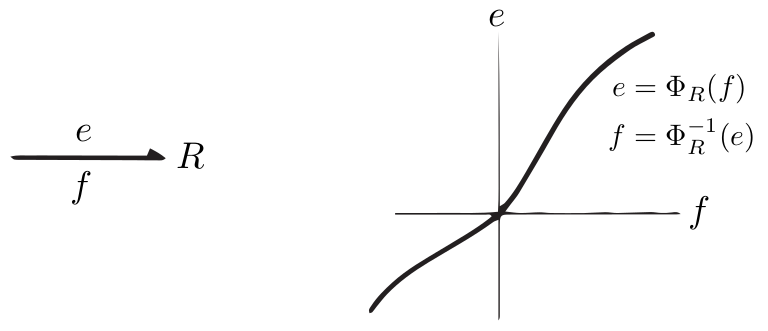
\includegraphics[width=0.8\textwidth]{1portR1}
\end{center}

\begin{center}
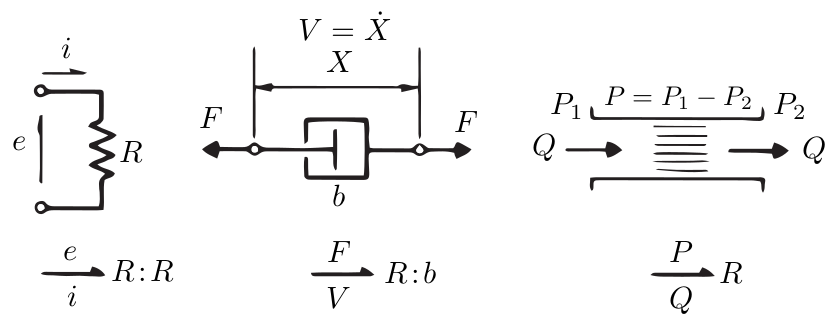
\includegraphics[width=0.8\textwidth]{1portR2}
\end{center}

















\end{document}
